\documentclass[]{article}

\begin{document}

\title{Deleted Text}

%50-70\% of the stars in globular clusters belong to the second population \citep{Carretta:2009kr}.

%The extent of the observed Na-O anti-correlation is strongly correlated with GC mass \citep{Conroy:2012eg}.

%\citet{Carretta:2006gb} find a correlation between light element anomalies and orbital parameters.

%\citet{Bekki:2006fh} propose that GCs form in dark matter halos surrounding dwarf galaxies.

%\citet{Conroy:2011ck} avoid the need for large initial GC masses by forming the second generation from a mixture of AGB ejecta and ambient ISM. This model predicts too small a number of anomalous stars, since the mass is dominated by material with normal abundances.

%The metallicity spread in GCs is larger than would be predicted by models of self-enrichment \citep{Bailin:2009du}.

%High precision photometry has revealed that the `simple' populations of globular clusters are in fact multiple populations \citep[e.g.,][]{Bedin:2004hn,Piotto:2007br,Milone:2008dz}. To date, multiple populations have been found in every globular cluster that has been studied with the sensitivity required to detect them.

$\omega$ Centauri ($\omega$ Cen, NGC 5139) is the brightest and most massive globular cluster in our galaxy. It is unusual for its size, as well as for having a large spread in metallicity \citep{Freeman:1975jf} and an age spread of several gigayears \citep{Smith:2000cb}. One indication of the large age spread is the chemical contribution from low-mass stars ($<4$ \Msun), which evolve too slowly ($>300$ megayears) to be relevant for most globular clusters

M22 (NGC 6656) is another globular cluster with an the intrinsic spread in metallicity \citep{Pilachowski:1982jg,Lehnert:1991ij}. The metallicity variation is smaller than in $\omega$ Cen, with [Fe/H] values ranging from -1.87 to -1.44 \citep{AlvesBrito:2012hy}. It has been suggested that M22 might have similar origins to $\omega$ Cen \citep{DaCosta:2009jl,DaCosta:2011jh}.

Of the globular clusters without metallicity variation, M4 (NGC 6121) and M5 (NGC 5904) are two that have very similar mean metallicities; their $\left<[\text{Fe/H}]\right>$ values are -1.08 for M4, and -1.21 for M5 \citep{Ivans:2001ju}. However, despite this, the [X/Fe] abundances Si, Al, Ba, and La, which are constant within each cluster, are overall about 0.3 dex higher in M4 relative to M5 \citep{Yong:2008in}.

\citet{Yong:2008in} derived an empirical \sprocess distribution by subtracting the abundances of the r-only cluster M5 from the r+s cluster M4. A similar distribution was found when \citet{Roederer:2011hw} subtracted the abundances of stars in the r-only group in M22 from those of the r+s group in the same cluster.

\subsection{The \textit{s}-process in massive stars}
The \textit{s}-process also takes place in massive stars during their pre-supernova evolution and possibly also during the supernova itself. By definition, massive stars are those that proceed through every core burning phase up to the formation of an Fe-core, which occurs for initial masses greater than about 12 \Msun. Massive stars are responsible for the `weak' \textit{s}-process component that mostly affects elements from Fe to Sr \citep{Beer:1992jv, Pignatari:2010ir}.

In massive stars, neutrons are released via the $\iso{22}{Ne}(\alpha,n)\iso{25}{Mg}$ reaction \citep{Peters:1968bf} during convective core He-burning and shell He- and C-burning \citep{The:2007gb}. As in intermediate-mass AGB stars, \iso{22}{Ne} is produced via He-burning of \iso{14}{N} left over from the H-burning CNO cycle. In non-rotating massive models, the \iso{14}{N} required for the \textit{s}-process is produced in small quantities and acts as a secondary element. Hence, there is very little \textit{s}-process production in non-rotating massive stars at very low metallicity.

In extremely low- and zero-metallicity massive stars, rotation increases the production of primary \iso{14}{N} by additional mixing \citep{Meynet:2006bh,Hirschi:2007br}. \iso{12}{C} from the He-burning core is transported to the H-burning shell where it is converted into \iso{14}{N}, then mixed back in the core and undoes two $\alpha$ captures.

Since some \iso{14}{N} is converted into the neutron-source \iso{22}{Ne}, rotation enhances \textit{s}-process production in low-metallicity massive stars \citep{Pignatari:2008ec}.

\begin{figure}
 \begin{center}\includegraphics[width=\textwidth]{figures/frischknecht2012-f1}\end{center}
 \caption{Production factors (ejected mass divided by the initial mass of the element) for 25 \Msun, $Z=10^{-5}$ models with and without rotation. CF88/10 denotes a model with a reduced $\iso{17}{O}(\alpha,\gamma)\iso{21}{Ne}$ rate (so the activity of $\iso{17}{O}(\alpha,n)\iso{21}{Ne}$ is relatively higher) to highlight the uncertainty related to the neutron poison \iso{16}{O}. From Figure 1 of \citet{Frischknecht:2012il}.}\label{fig:frischknecht2012-f1}
\end{figure}

\citet{Frischknecht:2012il} calculated heavy element yields from the first rotating massive models to include a full \textit{s}-process network. Their grid of models includes masses of 15, 20, 25, and 40 \Msun\ at low-metallicity ([Fe/H] of -5.8, -3.8 and -1.8) with several different rates of internal rotation. Figure \ref{fig:frischknecht2012-f1} shows the dramatic enhancement of \textit{s}-process yields with increasing rotation rate in a 25 \Msun, $Z=10^{-5}$ model. In Chapter \ref{chap:shinglesetal2014}, we apply these yields to a globular cluster chemical evolution model.

\subsection{Stellar modelling uncertainties}

The yields of \textit{s}-process elements in AGB stars are sensitive to many uncertainties including mass-loss rates, and the numerical treatment of convection, the partially mixed zone, and nuclear reaction rates.

In both AGB stars and massive stars, the \textit{s}-process production depends on the rate of the $\iso{22}{Ne}(\alpha,n)\iso{25}{Mg}$ reaction \citep{Longland:2012ix}. The \iso{22}{Ne} neutron source has a high temperature sensitivity and is therefore subject to uncertainties in the temperature of the He-burning shell, which can be increased by the inclusion of convection overshoot into the CO core \citep{Herwig:2000ua}.

Once \textit{s}-process elements have been produced in the He-intershell, their presence in stellar spectra require them to be transported up to the stellar photosphere. In interpulse phase following thermal pulses on the AGB, the base of the envelope convection zone is predicted to move down into the He-intershell (Third Dredge-up or TDU) and mix nuclear burning products up to the stellar surface.

The efficiency of TDU is subject to debate, and depends on the treatment of convection in the stellar model. Models using the full spectrum of turbulence (FST) theory predict a shorter AGB phase with fewer thermal pulses than models using the mixing length theory (MLT) \citep{Ventura:2004dp}. FST models also predict a shallow TDU, and increase proton capture nucleosynthesis in the envelope compared to MLT models \citep{Ventura:2005fs}.

The choice of mass loss prescription strongly affects AGB stellar yields even when the remnant mass is known. Yields are obtained by integrating the stellar wind, and the wind composition varies to match the changing surface abundances during the AGB. A mass loss prescription that predicts a steady wind \citep[e.g.,][]{Reimers:1975vw} one in which mass is lost disproportionately over the last few thermal pulses \citep[e.g.,][]{Vassiliadis:1993jk} will result in different yield predictions from stellar models \citep{Stancliffe:2007er}.

In massive star models \iso{16}{O} acts as a neutron poison, efficiently absorbing free neutrons. The resulting $^{17}$O nuclei may re-release neutrons via $\iso{17}{O}(\alpha,n)\iso{21}{Ne}$ or prevent their release via $\iso{17}{O}(\alpha,\gamma)\iso{21}{Ne}$. The branching ratio between these two reactions is highly uncertain and strongly affects \textit{s}-process yields \citep{Frischknecht:2012il}.

Rotation also contributes significant uncertainties to stellar modelling. Not only is the distribution of rotation rates in early stars uncertain, but our understanding of the effects of rotation on stellar structure and evolution is a topic of ongoing research \citep{Langer:2012jy}.
%%%%%%%%%%%%%%%%%% END OF MODELLING UNCERTAINTIES

\begin{figure}
 \begin{center}\includegraphics[width=0.9\textwidth]{figures/roederer2011-f6}\end{center}
 \caption{Empirical \textit{s}-process distributions derived from M4 - M5 (above) and M22 (r+s) $-$ (r-only) (below). Figure from \citet{Roederer:2011hw}.}\label{fig:roederer2011-f6}
\end{figure}

\begin{figure}
 \begin{center}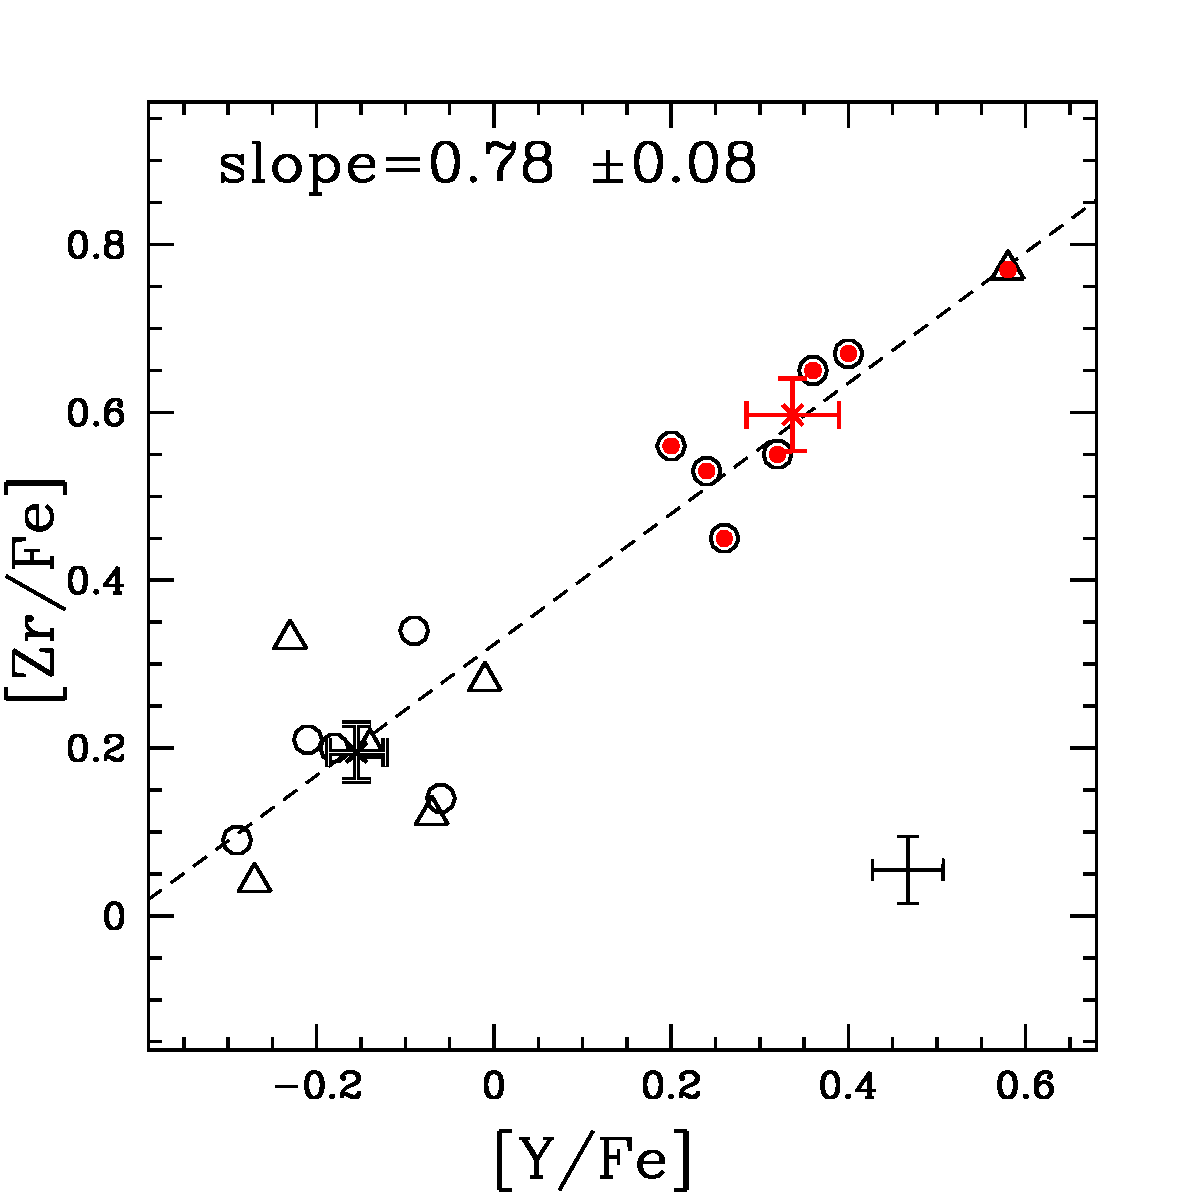
\includegraphics[width=0.33\textwidth]{figures/marino09-f7a}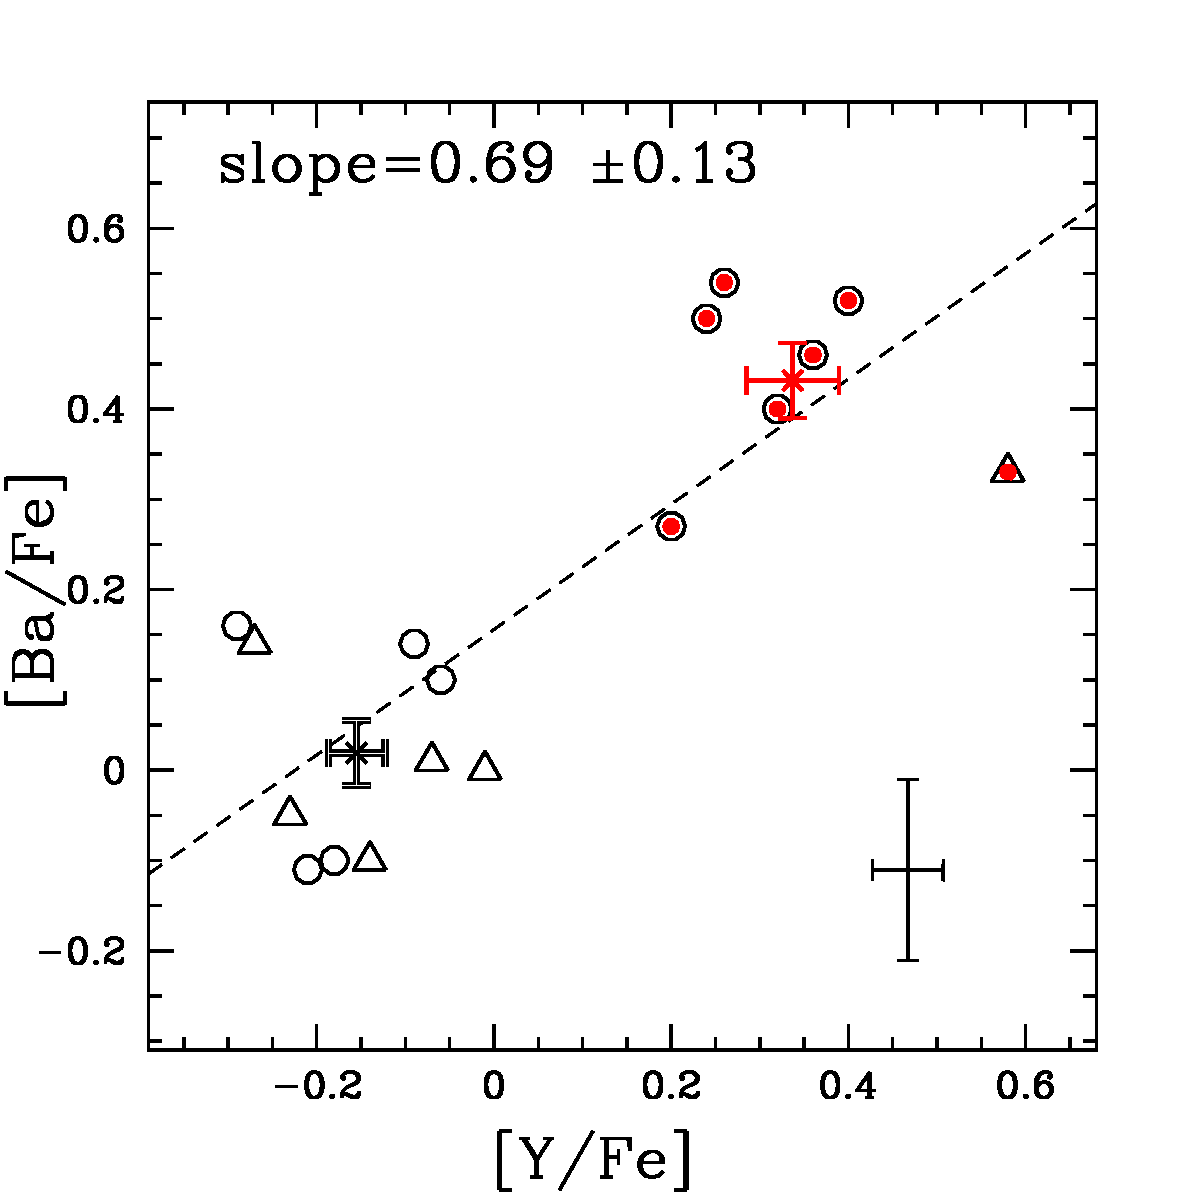
\includegraphics[width=0.33\textwidth]{figures/marino09-f7b}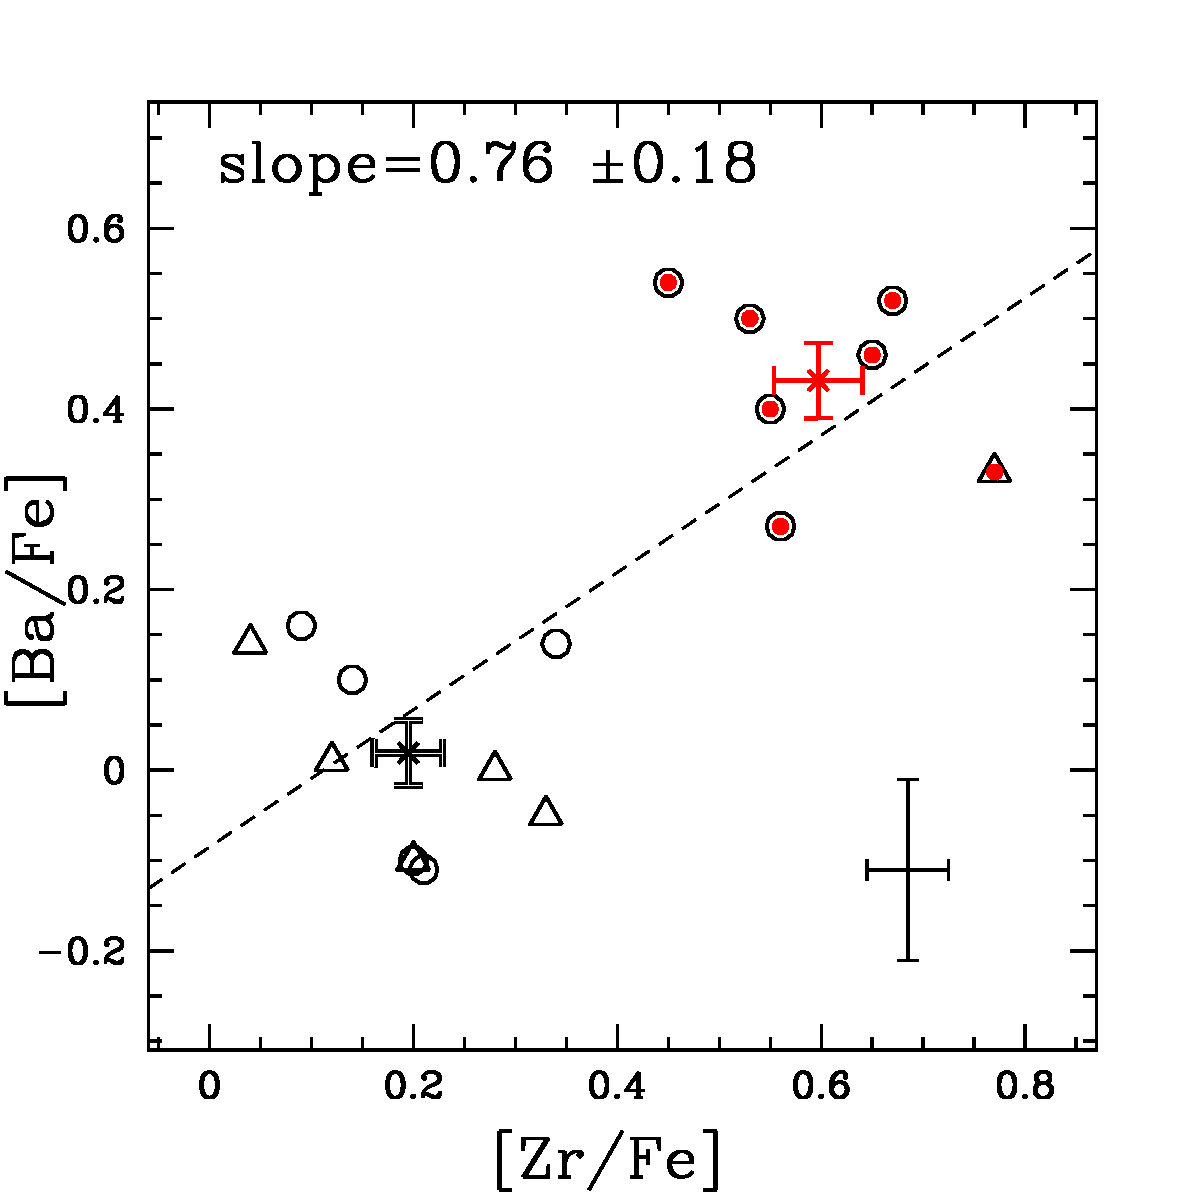
\includegraphics[width=0.33\textwidth]{figures/marino09-f7c}\end{center}
 \caption{$s$-Process abundances of the two groups in M22. Figure from from \citet{Marino:2009je}.}\label{fig:marino09-f7}
\end{figure}

\begin{figure}
 \begin{center}\includegraphics[width=\textwidth]{figures/gratton2004-f12.jpg}\end{center}
 \caption{Abundances of stars in $\omega$ Centauri. Filled symbols represent data from \citet{Norris:1995kc}; open symbols, data from \citet{Smith:2000cb}; crosses, data from \citet{Pancino:2002eq}. Figure from \citet{Gratton:2004dy}.}\label{fig:gratton2004-f12}
\end{figure}

\end{document}